\chapter{Công nghệ sử dụng}
\label{Chapter3}
\textit{Nội dung chương này sẽ đề cập đến các công nghệ sẽ được áp dụng bên trong hệ thống, các phần mềm , thư viện cần để hệ thống hoạt động, cách cài đặt các phần mềm và thư viện cần sử dụng. }

%thư viện requests
\section{Thư viện Requests}
\subsection{Định nghĩa }

Requests là một thư viện trong Python sử dụng để gửi các request HTTP. Request HTTP sẽ trả về một Respond Object với tất cả dữ liệu như nội dung, trạng thái, mã hoá, ... 

Việc sử dụng Requests trong đề tài này là dùng cho việc scraping câu hỏi và câu trả lời pháp luật từ website hỏi đáp pháp luật.

Để tạo một GET request thì chỉ cần import tất cả thư viện của module vào và thực hiện yêu cầu. Ví dụ như là:

\begin{lstlisting}
	import requests
	req = requests.get('https://hoidap.thuvienphapluat.vn/')
\end{lstlisting}

Tất cả các thông tin về yêu cầu của chúng ta bây giờ được lưu trữ trong một đối tượng Response được gọi là req. Vì vậy, để có thể tìm được các thuộc tính của trang web chỉ cần truy cập vào các thuộc tính của trang web có trong đối tượng req.

Việc phân tích, tìm kiếm thông tin trong đối tượng req cũng chính là nội dung chính của việc scraping data từ một website.

Thư viện này sẽ được áp dụng vào trong bài toán thu thập dữ liệu câu hỏi và câu trả lời về Pháp luật ở website cung cấp thông tin về Pháp luật.
%BeautifulSoup
\section{Thư viện BeautifulSoup}

BeautifulSoup\cite{Scraping} là một thư viện của Python nhằm hỗ trợ để bóc tách dữ liệu ra khỏi các file HTML. Nó hoạt động cùng với các \textbf{parser} để điều hướng, tìm kiếm, chỉnh sửa trong parse tree. Các parser khác nhau như là: html.parser, lxml, html5lib.

Parser \textbf{lxml} là một loại parser hỗ trợ trong việc phân tích HTML để phục vụ cho công việc scraping dữ liệu.

Các Object cần quan tâm khi sử dụng BeautifulSoup là:
\begin{itemize}
	\item Tag: tương ứng với một thẻ tag trong tài liệu HTML.
	\item NavigableString: là một chuỗi tương ứng với một bit văn bản có chứa trong một tag.
	\item BeautifulSoup: là một đối tượng đại diện cho toàn bộ tài liệu.
	\item Comment: là một dạng đặc biệt của NavigableString, cho phép truy cập vào các comment của một file HTML.
\end{itemize}

Thư viện này sẽ được áp dụng vào trong bài toán thu thập dữ liệu câu hỏi và câu trả lời về Pháp luật ở website cung cấp thông tin về Pháp luật.
%Python Vietnamese Toolkit
\section{Phân tách từ bằng Python Vietnamese Toolkit}
\subsection{Định nghĩa PyVi}
Python Vietnamese Toolkit(PyVi)\cite{pyvi} là một công cụ xử lý ngôn ngữ tự nhiên dùng cho tiếng Việt với các hàm xử lý như:

\begin{itemize}
	\item Tokenization: tách từ, cụm từ trong văn bản
	\item POS tagging: gán nhãn từ loại, các loại từ bao gồm: A – Adjective: tính từ, C – Coordinating conjunction: liên từ, E – Preposition: giới từ, I – Interjection: thán từ,L – Determiner: từ hạn định, M – Numeral: số, N - Common noun: danh từ chung, Nc - Noun Classifier: phân loại danh từ, Ny - Noun abbreviation: các danh từ viết tắt, Np - Proper noun: danh từ riêng, Nu - Unit noun: danh từ đơn vị, P – Pronoun: đại từ, R – Adverb: trạng từ, S - Subordinating conjunction:  liên từ phụ thuộc, T - Auxiliary, modal words: động từ khiếm khuyết, V – Verb: động từ, X – Unknown: các từ không xác định được, F - Filtered out (punctuation): các từ được lọc ra bởi dấu chấm câu
	\item Accents removal: bỏ dấu từ
	\item Accents adding: thêm dấu từ
	
\end{itemize}

\begin{figure*}[htp]
    \centering
    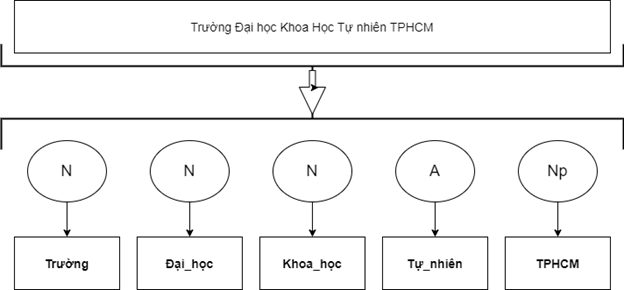
\includegraphics[scale=0.7]{images/pyvi_segment}
    \caption{Minh hoạ tách từ bằng PyVi.}
    \label{fig:ex_pyvi_1}
\end{figure*}
\pagebreak
\subsection{Tính năng chính của PyVi}
Sau đây là một đoạn code mẫu mô tả cách sử dụng và kết quả trả về của PyVi:
%biện pháp thay thế cho code bị lỗi encode utf-8
\begin{figure*}[htp]
	\centering
	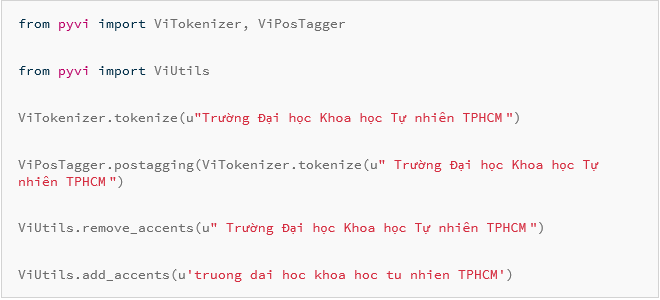
\includegraphics[scale=0.85]{images/pyvi_demo_code}
\end{figure*}

\hfill 

Khi chạy đoạn code trên, ta sẽ thu được các kết quả như:

Tokenize (tách từ):

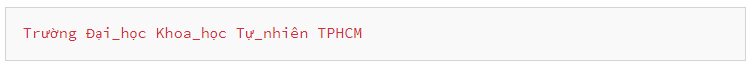
\includegraphics[scale=0.7]{images/segment1}

POS\_tagging (gán nhãn từ loại): khi thực hiện POS tagging thì hàm sẽ thực hiện tách từ (Tokenize) trước khi trả về kết quả. Kết quả trả về gồm mảng 2 chiều với thứ tự gán nhãn tương ứng với nhau:

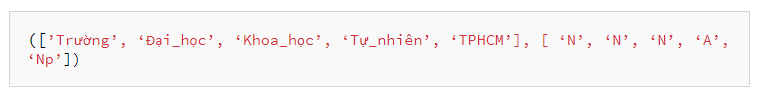
\includegraphics[scale=0.7]{images/segment2}

Accents removal (bỏ dấu):

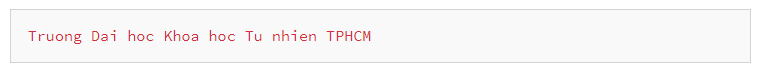
\includegraphics[scale=0.7]{images/segment3}

Accents adding(Thêm dấu):

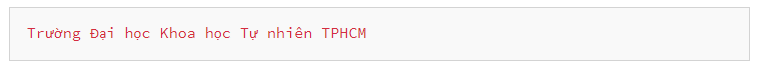
\includegraphics[scale=0.7]{images/segment4.png}

Thư viện này sẽ được áp dụng vào trong bài toán xử lý ngôn ngữ tự nhiên(tách từ ghép trong tiếng Việt).
%transformer
\section{Mô hình Transformer}
\subsection{Định nghĩa mô hình Transformer}
Trước khi Transformers xuất hiện, đa số các tác vụ xử lý ngôn ngữ tự nhiên sử dụng kiến trúc của Recurrent Neural Networks(RNNs) – Mạng nơ-ron hồi quy. Điểm yếu của RNNs là khó nắm bắt được sự phụ thuộc xa giữa các từ trong câu và tốc độ huấn luyện mô hình chậm do phải xử lý tuần tự. Transformers có thể giải quyết các vấn đề này.

Transformers ra đời nhằm giải quyết vấn đề chuyển đổi chuỗi dữ liệu hoặc dịch máy, chẳng hạn như các bài toán như nhận dạng giọng nói, chuyển văn bản thành giọng nói,…
	
Kiến trúc của Transformers bao gồm hai phần là Encoder và Decoder, Encoder dùng để học, chuyển hoá vector biểu diễn của câu văn bản và Decoder sẽ thực hiện biểu diễn vector dó dưới ngôn ngữ của người dùng.

\pagebreak
\subsection{Ưu điểm của Transformers}
Ưu điểm của Transformers là mô hình này có khả năng xử lý song song cho các từ trong câu văn bản, gia tăng hiệu suất và giảm thời gian huấn luyện.

\begin{figure*}[htp]
    \centering
    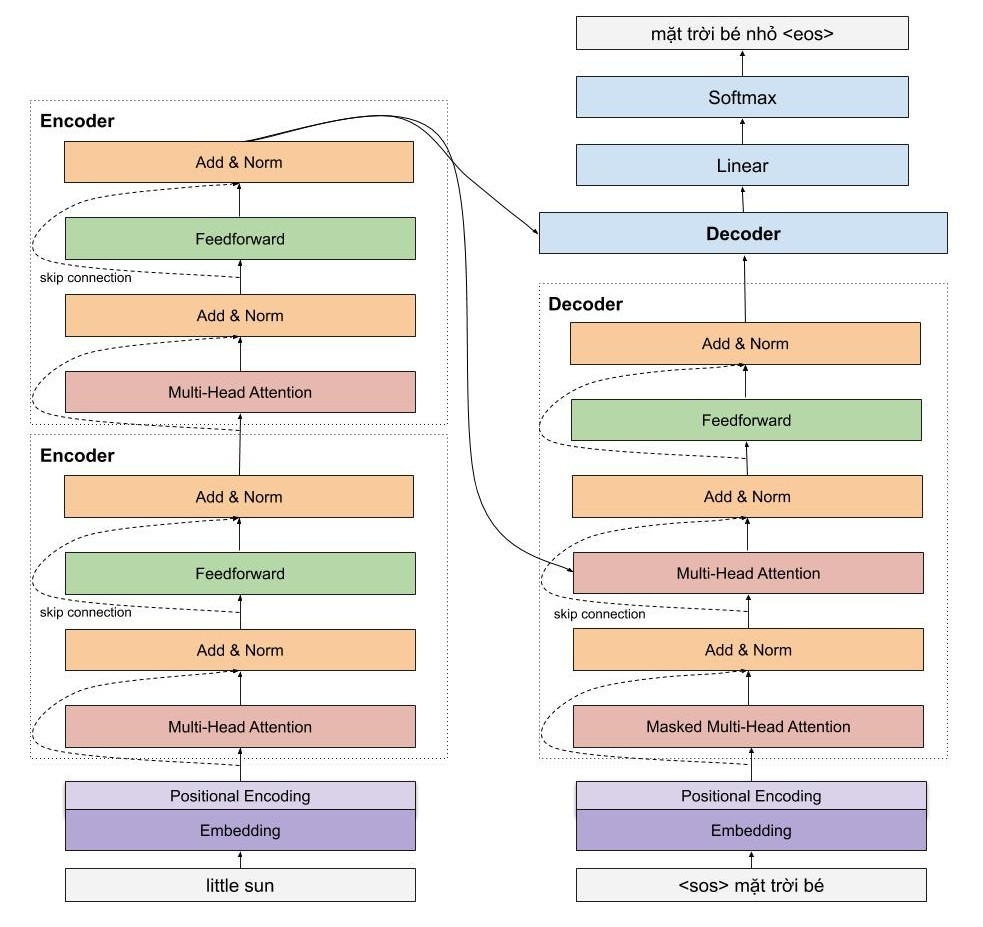
\includegraphics[width=13 cm, height=15 cm]{images/transformer_schema}
    \caption{Mô hình tổng quát của cấu trúc của Transformer.}
    \label{fig:transformer_schema}
\end{figure*}


Ý tưởng của mô hình Transformers là áp dụng cơ chế Attention. Chính thành phần Multi-Head Attention trong các lớp Encoder cho phép mô hình mã hoá một từ có thể sử dụng thông tin của những từ liên quan đến nó.

Mô hình này sẽ được áp dụng vào trong bài toán mã hoá dữ liệu câu hỏi Pháp luật.
\pagebreak


%BERT MODEL

\section{Mô hình BERT}
\subsection{Định nghĩa mô hình BERT}
BERT là viết tắt của “Bidirectional Encoder Representations from Transformers”, là một mô hình học sẵn, học biểu diễn vector đại diện cho câu theo ngữ cảnh 2 chiều.

Một trong những khó khăn khi xử lý ngôn ngữ tự nhiên đó là việc thiếu hụt dữ liệu gán nhãn. Hầu hết các dữ liệu đều được gán nhãn thủ công bởi con người, vì vậy, số lượng mẫu dữ liệu chất lượng không nhiều. Do đó, để giải quyết vấn đề này, các mô hình xử lý ngôn ngữ tự nhiên sử dụng cơ chế tiền xử lý dữ liệu, cơ chế này tạo ra một mô hình chung được huấn luyện từ số lượng lớn dữ liệu không gán nhãn, chẳng hạn như các mô hình Word2Vec, Glove,… Tuy nhiên, các mô hình này thường không biểu diễn chính xác ngữ nghĩa của từ trong ngữ cảnh câu văn bản, dẫn đến khó khăn trong việc xác định nghĩa của một từ đang được đề cập trong ngữ cảnh nào.

BERT có khả năng tạo ra mô hình ngôn ngữ cho phép các hệ thống tìm kiếm hiểu rõ hơn về ngữ nghĩa của từ trong câu dựa vào xem xét mối liên hệ giữa các từ trước và sau của từ đó.  

BERT được xây dựng dựa trên Transformers với hai biến thể:
\begin{itemize}
    \item BERT$_{BASE}$ gồm 12 lớp Encoder, kích thước của các lớp ẩn là 768 với 110 triệu tham số. 
    \item BERT$_{LARGE}$ gồm 24 lớp Encoder, kích thước của các lớp ẩn là 1024 với 340 triệu tham số
\end{itemize}
\begin{figure*}[htp]
    \centering
    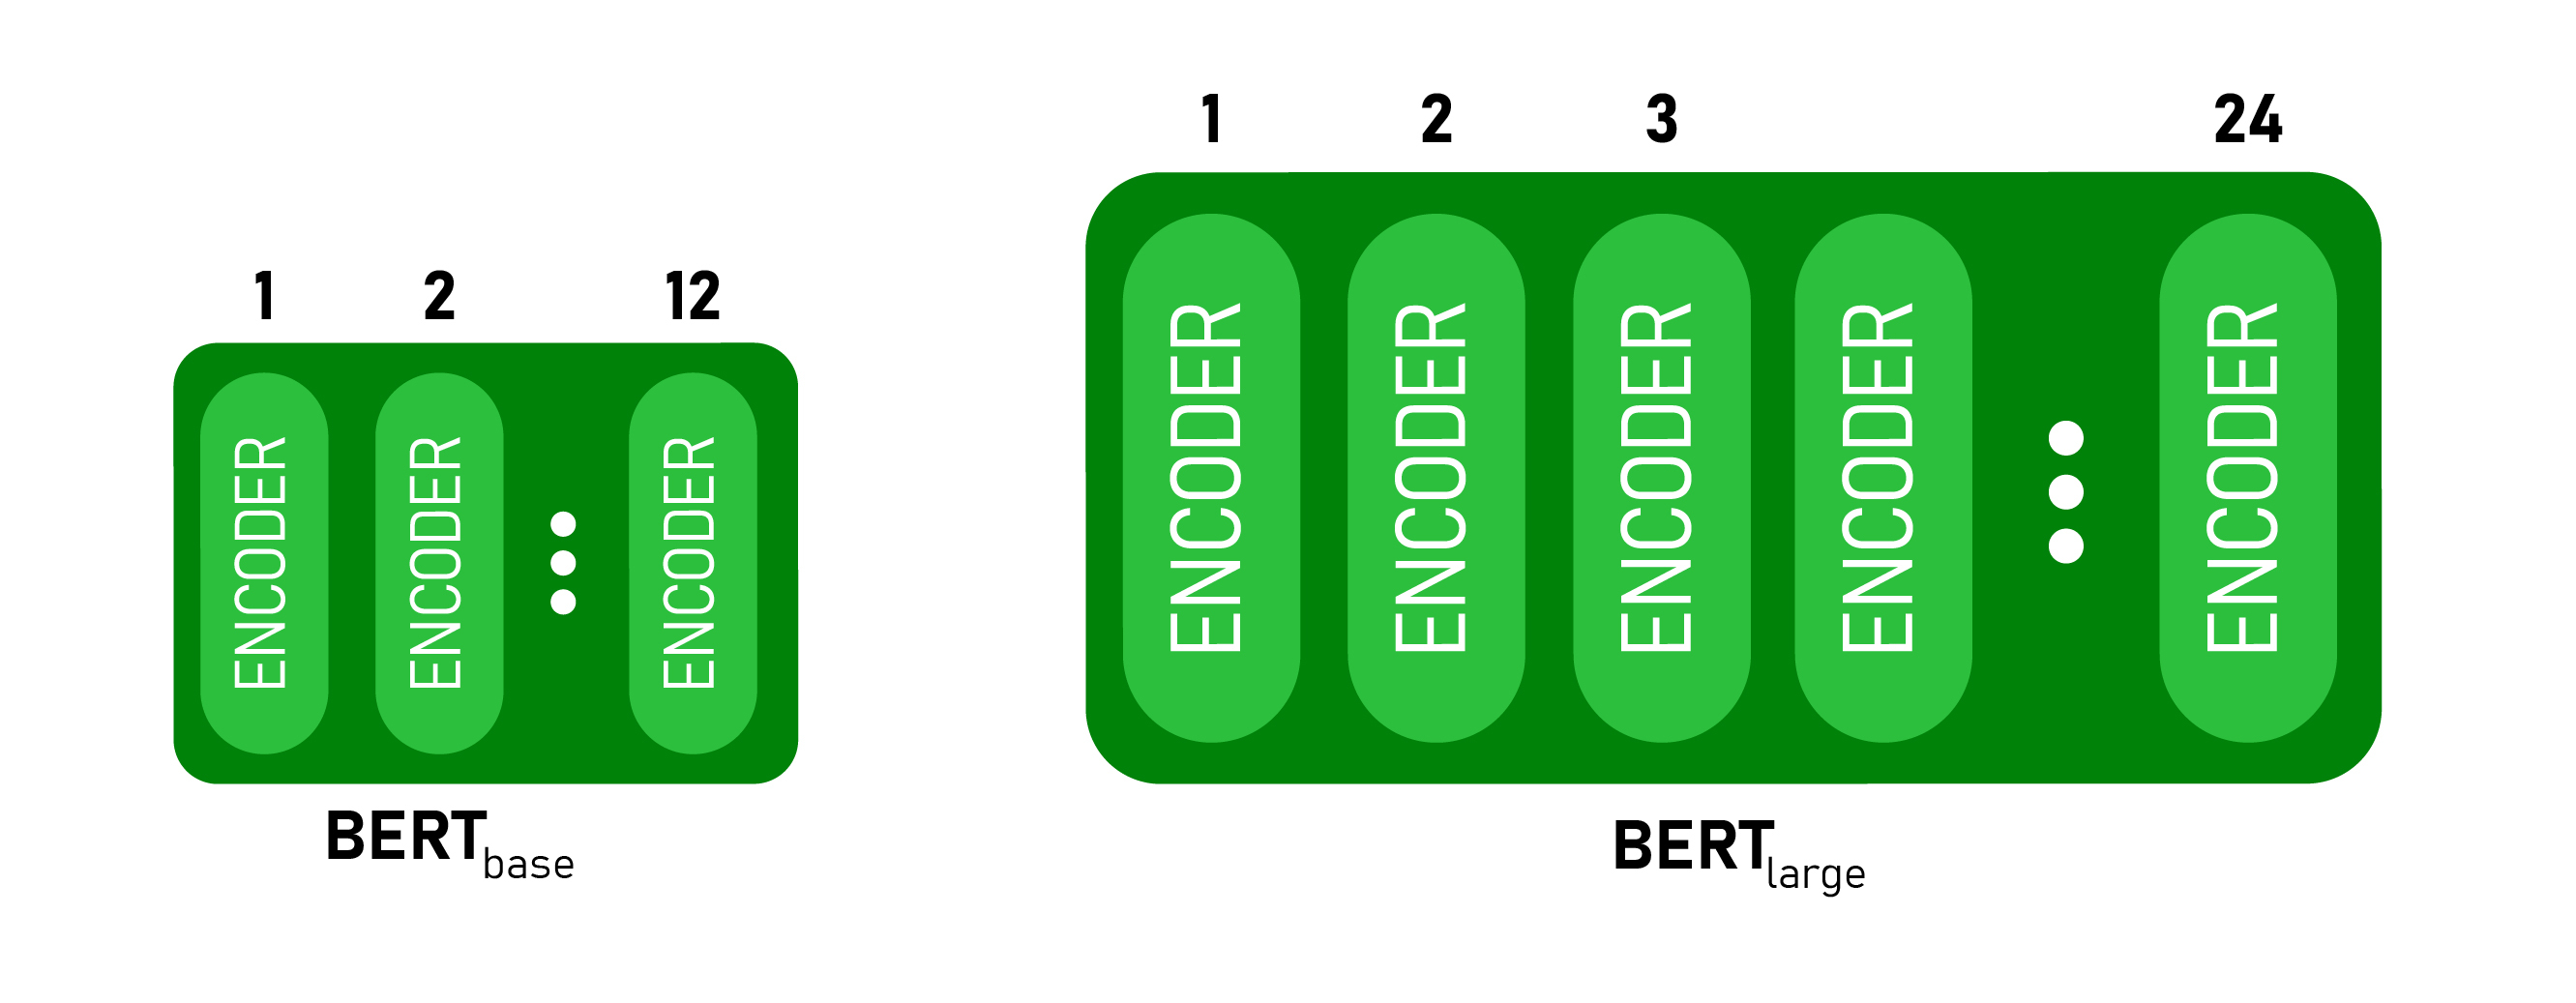
\includegraphics[scale=0.1]{images/bert-base-and-large.jpg}
    \caption{Kích thước của 2 dạng BERT.}
    \label{fig:BERT_SIZE}
\end{figure*}

Trong khi đó kiến trúc của Transformers chỉ có 6 lớp Encoder, cho thấy khả năng xử lý của BERT mang lại hiệu suất cao hơn.
\begin{figure*}[htp]
    \centering
    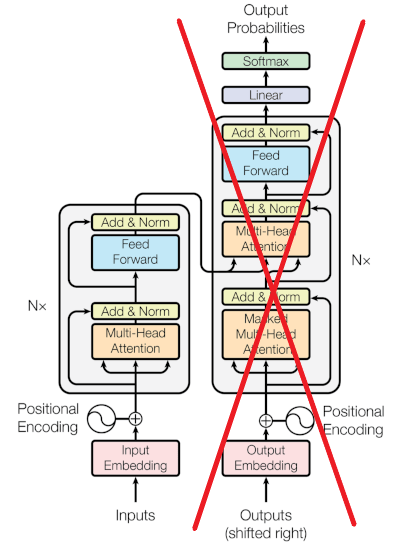
\includegraphics[width=12.5 cm, height=17 cm]{images/encode_bert.png}
    \caption{Encode BERT.}
    \label{fig:encode_bert}
\end{figure*}


Kiến trúc của BERT khác với Transformers ở chỗ nó chỉ dùng thành phần Encoder của Transformers vì mục tiêu sử dụng BERT là để tạo ra được một mô hình thực hiện các tác vụ NLP khác nhau. Việc sử dụng Encoder cho phép BERT mã hóa thông tin ngữ nghĩa, cú pháp của câu trong quá trình nhúng. 

BERT không sử dụng thành phần Decoder của Transformers nên kết quả đầu ra của nó là một embedding – một không gian vector dùng để biểu diễn dữ liệu có thông tin về mối liên hệ, sự tương đồng về mặt ngữ nghĩa, ngữ cảnh của dữ liệu, trong đó bao gồm nhiều chiều và các từ có sự tương đồng sẽ có vị trí gần nhau. Vì kết quả đầu ra của BERT là word embedding nên người sử dụng có thể làm các tác vụ khác nhau. Người dùng có thể sử dụng các kỹ thuật để tính sự tương đồng, chẳng hạn như Cosine Similarity để so sánh giữa các vector đại diện và trả về điểm số tương đồng.

Mô hình này sẽ được áp dụng vào trong bài toán mã hoá dữ liệu câu hỏi Pháp luật.
%Sentence-transformer
\section{Sentence-transformer}
Sentence Transformers\cite{sentencetransformer} là 1 framework dùng để Embedd (nhúng) những câu văn, đoạn văn, hình ảnh để tạo ra các Embeddings có ý nghĩa về mặt ngữ nghĩa, được sử dụng để áp dụng cho các bài toán, ứng dụng Semantic Search (tìm kiếm ngữ nghĩa) hoặc là Multi-lingual Zero-shot Classification (phân loại Zero-shot đa ngôn ngữ).

Sentence Transformers là phương pháp để tính toán, tạo ra các vector biểu diễn cho các câu văn, đoạn văn bản hay là một hình ảnh. Các mô hình như BERT, RoBERTa, XLM-RoBERTa,... đều dựa trên framework Sentence Transformers này. Các đoạn văn bản sau khi được Vector hóa có thể tìm được sự tương đồng về mặt ngữ nghĩa với nhau bằng cách dùng phương pháp tính Cosine Similarity.

Như vậy với Sentence Transformers, ta có thể:

Dùng các độ đo khoảng cách hoặc góc để tính độ tương đồng về ngữ nghĩa của các câu, áp dụng để phân nhóm câu theo ngữ nghĩa (Semantic Clustering), dùng trong Hệ thống truy vấn thông tin theo ngữ nghĩa (Semantic Information Retrieval), tính toán câu tương tự (Computing Sentence Similarity), ...

Sử dụng như Pre-trained Model trong các Transfer Learning, đã có hơn 100 ngôn ngữ được huấn luyện sẵn nên rất dễ cho việc sử dụng.

\pagebreak
Ví dụ về sử dụng mô hình Sentence Transformer để nhúng (Embedd) các câu văn:
\begin{lstlisting}[language=python]
from sentence_transformers import SentenceTransformer
sentences = ["There was coal in his stocking and he was thrilled"]
model = SentenceTransformer('paraphrase-MiniLM-L6-v2')
embeddings = model.encode(sentences)
print("Sentence: ", sentences)
print("Embedding: ", embeddings)
\end{lstlisting}

Và đây là kết quả:
\begin{lstlisting}
Sentence:  ['There was coal in his stocking and he was thrilled']
	Embedding: [[-3.29191387e-01  1.03968787e+00 -2.23834172e-01  7.96381384e-02
	-7.98925042e-01 -1.18792735e-01  7.98527181e-01  3.68809402e-01
	-1.13197708e+00  9.99245495e-02 -5.30997992e-01 -2.71604806e-01
	-1.89905569e-01 -7.41842622e-03 -3.44552487e-01  5.15601277e-01...]]	
\end{lstlisting}

%Phở bert
\section{Mô hình PhoBERT}

PhoBERT\cite{PhoBERT},\cite{PhoBERT_VNMESE}  là một pre-trained model dựa trên BERT, được xây dựng để huấn luyện riêng cho ngôn ngữ tiếng Việt, dựa trên kiến trúc RoBERTa – model tương tự BERT nhưng có phần tối ưu quá trình tiền huấn luyện cho hiệu suất cao do kiến trúc này đã bỏ đi tác vụ Next Sentence Prediction. 

PhoBERT cũng có hai kích thước là PhoBERT$_{BASE}$ với 12 transformers block và PhoBERT$_{LARGE}$ với 24 transformers block. PhoBERT được huấn luyện từ 20GB dữ liệu về Tiếng Việt bao gồm 1GB Vietnamese Wikipedia corpus và 19GB Vietnamese news corpus. 

PhoBERT sử dụng RDR Segmenter của VnCoreNLP để tách từ cho dữ liệu đầu vào trước khi qua BPE encoder. PhoBERT tượng tự BERT, chỉ khác là dùng cho việc xử lý ngôn ngữ tiếng Việt nên kiến trúc của PhoBERT cũng thừa hưởng thành phần Encoder của mô hình Transformers, không bao gồm Decoder.

Mô hình này sẽ được áp dụng vào trong bài toán mã hoá dữ liệu câu hỏi Pháp luật.
%SimCSE
\section{Pre-trained model SimCSE}

SimCSE\cite{gao2021simcse} là một pre-trained model sử dụng PhoBERT, dùng để mã hóa câu, đoạn văn bản dữ liệu đầu vào. SimCSE cho hiệu suất huấn luyện cao hơn, làm việc đồng thời với cả hai loại dữ liệu đã được gắn nhãn hoặc không.

Việc áp dụng mô hình SimCSE là cần thiết vì đây là mô hình sử dụng các phương pháp kỹ thuật hiện đại nhất trong tác vụ xử lý dữ liệu đầu vào. Thêm vào đó, với tác vụ đánh giá sự tương đồng ngữ cảnh giữa các câu văn bản, SimCSE mang lại kết quả khá cao so với BERT.

Mô hình này sẽ được áp dụng vào trong bài toán mã hoá dữ liệu câu hỏi Pháp luật.
%Elasticsearch
\section{Elasticsearch}
Elasticsearch là một công cụ tìm kiếm dựa trên nền tảng Apache Lucene. Nó cung cấp một bộ máy tìm kiếm dạng phân tán, có đầy đủ công cụ với một giao diện web HTTP có hỗ trợ dữ liệu JSON.

Elasticsearch chạy trên server riêng và đồng thời giao tiếp thông qua RESTful do vậy nên nó không phụ thuộc vào client viết bằng gì hay hệ thống hiện tại của bạn viết bằng gì. Nên việc tích hợp nó vào hệ thống bạn là dễ dàng, bạn chỉ cần gửi request http lên là nó trả về kết quả.

Các khái niệm cần phải biết khi sử dụng Elasticsearch\cite{ES} là:
\begin{itemize}
	\item Document: là một Object JSON, có thể xem là đơn vị lưu trữ nhỏ nhất của Elasticsearch
	\item Index: được xem như là một "database" khi quy chiếu sang với cơ sở dữ liệu quan hệ.
	\item Shard: là khối các Elasticsearch với mục đích mở rộng, nâng cấp.
	\item Node: Là trung tâm hoạt động của Elasticsearch. Là nơi lưu trữ dữ liễu ,tham gia thực hiện đánh index của cluster cũng như thực hiện các thao tác tìm kiếm.
	\item Cluster: là tập hợp các nodes hoạt động cùng với nha. Mỗi Cluster có một Node chính được chọn một cách tự động và có thể thay thay thế nếu có sự cố xảy ra.
\end{itemize}

Chức năng chính của Cluster đó chính là quyết định xem shards nào được phân bổ cho node nào và khi nào thì di chuyển các Cluster để cân bằng lại Cluster.

\subsection{Ưu điểm của Elasticsearch}
Tìm kiếm dữ liệu rất nhanh chóng, mạnh mẽ dựa trên Apache Lucene ( near-realtime searching)

Có khả năng phân tích dữ liệu (Analysis data)

Khả năng mở rộng theo chiều ngang

Hỗ trợ tìm kiếm mờ (fuzzy), tức là từ khóa tìm kiếm có thể bị sai lỗi chính tả hay không đúng cú pháp thì vẫn có khả năng Elasticsearch trả về kết quả tốt.

Hỗ trợ Structured Query DSL (Domain-Specific Language ), cung cấp việc đặc tả những câu truy vấn phức tạp một cách cụ thể và rõ ràng bằng JSON.

Hỗ trợ nhiều Elasticsearch client như Java, PhP, Javascript, Ruby, .NET, Python

\subsection{Nhược điểm của Elasticsearch}

Elasticsearch được thiết kế cho mục đích search, do vậy với những nhiệm vụ khác ngoài search như CRUD thì elastic kém thế hơn so với những database khác như Mongodb, Mysql …. Do vậy người ta ít khi dùng Elasticsearch làm database chính, mà thường kết hợp nó với 1 database khác.

Trong Elasticsearch không có khái niệm database transaction , tức là nó sẽ không đảm bảo được toàn vẹn dữ liệu trong các hoạt độngInsert, Update, Delete.Tức khi chúng ta thực hiện thay đổi nhiều bản ghi nếu xảy ra lỗi thì sẽ làm cho logic của mình bị sai hay dẫn tới mất mát dữ liệu. Đây cũng là 1 phần khiến Elasticsearch không nên là database chính.

Không thích hợp với những hệ thống thường xuyên cập nhật dữ liệu. Sẽ rất tốn kém cho việc đánh index dữ liệu.	

%Flask
\section{Web Framework: Flask Framework}
\begin{enumerate}
    \item Flask Framework:
    \begin{figure*}[htp]
        \centering
        
\includegraphics{images/Flask_Logo}
        \caption{Flask logo.}
        \label{fig:flask_logo}
    \end{figure*}
    

Flask là một Web Frameworks, được xây dựng bằng ngôn ngữ lập trình Python.
         
Flask dựa trên bộ công cụ \textbf{Werkzeg WSGI} và template engine \textbf{Jinja2}:

\textbf{WSGI} (Web Server Gateway Interface): WSGI là Giao diện Cổng Máy chủ Web, WSGI mô tả cách máy chủ web giao tiếp với các ứng dụng web và cách các ứng dụng web có thể được kết nối với nhau khi xử lý một yêu cầu.

\textbf{Werkzeug}: Werkzeug là một bộ công cụ WSGI thực hiện các yêu cầu, đối tượng phản hồi và các chức năng tiện ích, cho phép xây dựng một Web Framework trên đó. Flask framework sử dụng Werkzeg làm một trong những cơ sở của nó.

\textbf{jinja2}: jinja2 là một template engine phổ biến cho Python, được sử dụng để hiển thị dữ liệu cho các trang web. Jinja2 cho phép chuyển các biến Python vào các HTML template – thuận tiện cho việc đổ dữ liệu từ Back End đến Front End.

Flask cung cấp các thư viện, công cụ, cơ chế để xây dựng các Website từ nhỏ đến lớn, từ đơn giản tới phức tạp như: các API nhỏ, trang blog, trang web thương mại điện tử,…
        
Flask thuộc loại Micro-framework: có ưu điểm là rất nhẹ và nhỏ, không phụ thuộc vào thư viện bên ngoài nên rất ít lỗi, do đó dễ dàng đề phòng, phát hiện và xử lý các lỗi bảo mật
    
    
\item Ví dụ web API đơn giản xây dựng bằng Flask\cite{FlaskAPIWeb}:
Sau đây là một đoạn code để tạo một Route của một website

%code        
\begin{lstlisting}[language=Python]
from flask import Flask 
app = Flask(__name__) 
@app.route('/hello') 
def hello_world(): 
	return 'Hello, World!' 
if __name__ == '__main__': 
	app.run(host='0.0.0.0', port=5001)
\end{lstlisting}
    
Để khởi tạo instance của class, dòng code dưới sẽ tạo một web server điều hướng các request từ client đến ứng dụng của chúng ta, nó cũng là chính là một ứng dụng WSGI(Web Server Gateway Interface):
%code
\begin{lstlisting}[language=Python]
    app = Flask(__name__):
\end{lstlisting}

Route decorator cho FLask biết được url nào ứng với hàm nào, Web Server dựa vào đường dẫn và route decorator để chuyển yêu cầu tới hàm xử lý tương ứng $ hello\_world()$, hàm này đóng vai trò làm ứng dụng web (web application).
        
\begin{lstlisting}[language=Python]
    @app.route('/hello') 
\end{lstlisting}

Flask app được chạy với lệnh app.run(). Các tham số trong hàm run:

\begin{lstlisting}
    if __name__ == '__main__': 
	    app.run(host='0.0.0.0', port=5001)
\end{lstlisting}

	\textbf{Host= $'0.0.0.0'$}: Địa chỉ IP để ứng dụng Flask lắng nghe các kết nối, mặc định giá trị của tham số này là $'127.0.0.1'$ và ứng dụng flask chỉ chấp nhận các kết nối từ máy local. chuyển giá trị này thành $'0.0.0.0'$ để ứng dụng chấp nhận các kết nối từ bên ngoài.
	
	\textbf{port=5001}: Giá trị của port là một số nguyên, giá trị mặc định bằng 5001. Là cổng được mở trên máy mà ứng dụng Flask chạy, cần chọn cổng mà chưa được mở trên máy để tránh gặp lỗi khi chạy.
	


\end{enumerate}

%table 3
\section{Hướng dẫn cài đặt các phần mềm cần thiết}
\subsubsection{ElasticSearch}
Truy cập: \url{https://www.elastic.co/downloads/elasticsearch} và tải bản phù hợp với hệ điều hành tại mục Downloads:

\begin{figure*}[htp]
	\centering
	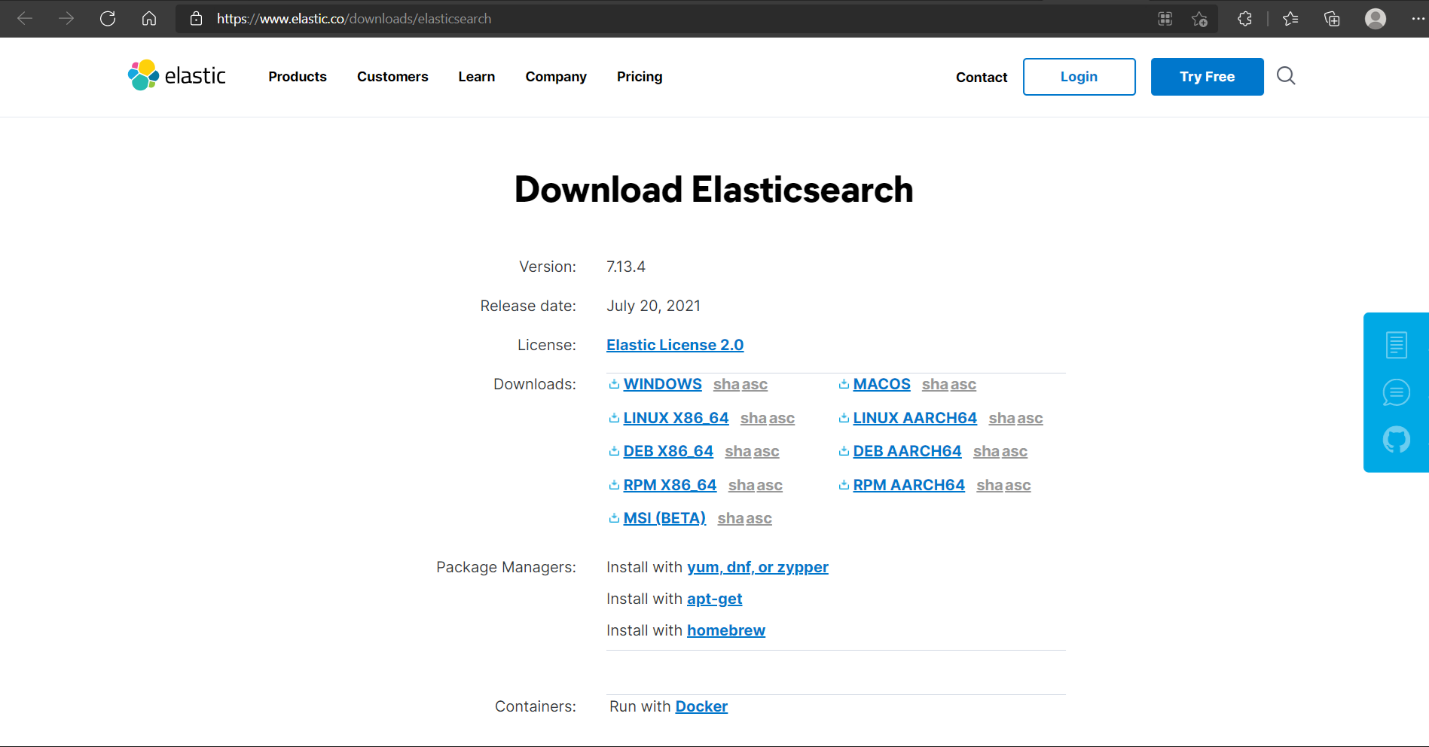
\includegraphics[scale=0.7]{images/elasticsearch1}
	\caption {Giao diện tải về Elastic search.}
	\label{fig:elasticsearch1}
\end{figure*}

Giải nén file .zip vừa tải về thành công ta được thư mục tương ứng

Vào thư mục giải nén:  bin và chạy file elasticsearch.bat

Mở trình duyệt truy cập: \url{http://localhost:9200/} để kiểm tra ElasticSearch đã chạy hay chưa, nếu thành công:

\begin{figure*}[htp]
	\centering
	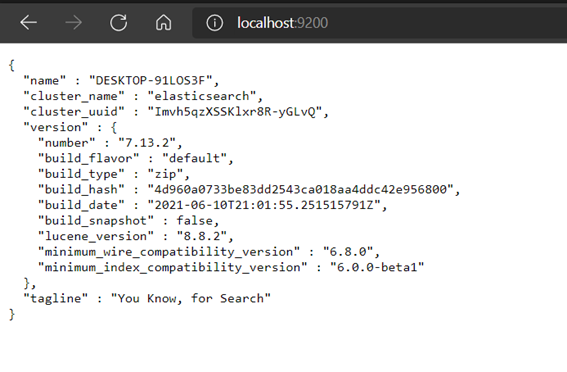
\includegraphics[scale=0.8]{images/elasticsearch2}
	\caption{Trả về kết quả là Elastic search được cài đặt thành công và đang hoạt động.}
\end{figure*}

\subsubsection{Cài đặt các thư viện cần thiết}
\textbf{BeautifulSoup}
\begin{lstlisting}
	pip install beautifulsoup4
\end{lstlisting}

\textbf{Flask 2.0.1}
\begin{lstlisting}
	pip install Flask
\end{lstlisting}

\textbf{utils 1.0.1}
\begin{lstlisting}
	pip install utils
\end{lstlisting}

\textbf{pandas 1.3.1}
\begin{lstlisting}
	pip install pandas
\end{lstlisting}

\textbf{elasticsearch}
\begin{lstlisting}
	pip install elasticsearch
\end{lstlisting}

\textbf{sentence-transformers 2.0.0}
\begin{lstlisting}
	pip install sentence-transformers
\end{lstlisting}

\textbf{pyvi 0.1.1}
\begin{lstlisting}
	pip install pyvi
\end{lstlisting}

\textbf{sklearn}
\begin{lstlisting}
	pip install sklearn
\end{lstlisting}

\textbf{numpy}
\begin{lstlisting}
	pip install numpy
\end{lstlisting}

\textbf{typing}
\begin{lstlisting}
	pip install typing
\end{lstlisting}

\textbf{requests}
\begin{lstlisting}
	pip install requests
\end{lstlisting}


Khi cài thành công các thư viện trên, khi import các thư viện vào trong hệ thống và chạy hệ thống sẽ không có báo lỗi xảy ra khi chạy.\newline

Trong 3 chương tiếp theo, nhóm sẽ tiếp tục trình bày rõ từng bước mà hệ thống sẽ thực hiện, hoạt động, kết quả của từng bước có trong hệ thống.